% =========================================================================
% Script-Aware Dual-Tokenization Fusion for Low-Resource Indic Scene Text
% Draft v2 (IJDAR submission) — 2026-07-12.
% Springer Nature template: compile on Overleaf against sn-jnl.cls
% (Springer Nature LaTeX template, two-column option), pdflatex.
% All numbers re-verified 2026-07-12 with verify_paper_numbers.py against
% the per-image prediction files in lstm_model/ (see README.md).
% FILL BEFORE SUBMISSION: author list, affiliation, email, funding.
% =========================================================================
\documentclass[iicol,pdflatex,sn-mathphys-num]{sn-jnl}

\usepackage{graphicx}
\usepackage{booktabs}
\usepackage{multirow}
\usepackage{amsmath,amssymb}
\graphicspath{{../figures/}}

\begin{document}

\title[Dual-Tokenization Fusion for Indic Scene Text]{Script-Aware
Dual-Tokenization Fusion in a Vision--Language Model for Low-Resource
Indic Scene-Text Recognition}

% ---- FILL: authors and affiliation --------------------------------------
\author*[1]{\fnm{Ritu} \sur{Baskey}}\email{baskeyritu@gmail.com}
%\author[1]{\fnm{FIRSTNAME} \sur{SURNAME}}   % co-author(s) TBD
\affil*[1]{\orgdiv{DEPARTMENT}, \orgname{INSTITUTION},
\orgaddress{\city{CITY}, \country{India}}}
% --------------------------------------------------------------------------

\abstract{Scene-text recognition for Indic scripts lags far behind English,
owing to scarce labeled data and to subword tokenizers that fragment
script-specific structures such as consonant conjuncts. We adapt a
vision--language model (Florence-2) to Bengali scene text and make its
tokenization \emph{script-aware} by injecting grapheme-cluster tokens,
improving word recognition from 52.4\% to 57.3\% on a leakage-free test
set. The BPE-tokenized and grapheme-tokenized decoders commit largely
\emph{complementary} errors, and a parameter-free fusion---selecting the
more confident decoder per image---outperforms both. The effect is not an
artifact of one language: under a single recipe with no per-language
tuning, fusion beats the better individual branch on every one of twelve
languages spanning nine Brahmic scripts and a Latin control (mean gain
$+5.0$ WRR, significant in all twelve; up to $+9.6$ on Tamil), and the
\emph{winning} branch flips with script coverage while the fusion gain
does not. A calibration analysis explains the mechanism: beam confidence
ranks correctness with AUROC 0.89--0.91, enabling the fusion rule,
selective prediction (91.4\% word accuracy at 50\% coverage), and a
cascade that retains 66--85\% of the fusion gain while invoking the second
decoder on only 27--58\% of images. With a grapheme-rarity-weighted
synthetic curriculum and confidence-filtered self-training, the full
system reaches 64.6\% word and 82.8\% character accuracy on our Bengali
test set and improves the public BSTD Bengali benchmark from 57.4\% to
62.1\%. On our independent test set the system is statistically
indistinguishable from a specialist PARSeq trained on ${\sim}1000\times$
more data. All data audits, negative results, and oracle ceilings are
reported.}

\keywords{Scene text recognition, Indic scripts, Grapheme clusters,
Tokenization, Vision--language models, Selective prediction}

\maketitle

\section{Introduction}\label{sec:intro}
Reading text in natural images is largely solved for Latin scripts but not
for the Brahmic scripts used by more than a billion people. Two obstacles
compound: (i)~\textbf{data scarcity}---public Bengali scene-text corpora
contain a few thousand labeled words, versus millions for English; and
(ii)~\textbf{tokenization mismatch}---modern vision--language models (VLMs)
inherit byte-pair-encoding (BPE) vocabularies trained mostly on Latin text,
which shatter Indic \emph{grapheme clusters} (e.g.\ conjuncts such as
\textit{ksha} or \textit{shri}) into fragments that are visually
meaningless, so the model must learn to reassemble units it never sees as
wholes.

This paper makes the tokenizer script-aware and then exploits the fact that
two differently-tokenized views of the same recognizer disagree in useful
ways. Our contributions:
\begin{enumerate}
  \item \textbf{Grapheme-aware VLM tokenization.} We inject Bengali
        grapheme-cluster tokens into Florence-2's tokenizer and fine-tune
        with LoRA; word recognition rate (WRR) rises 52.4\,$\to$\,57.3
        on our test set and 57.4\,$\to$\,59.8 on public BSTD Bengali.
  \item \textbf{Dual-tokenization confidence fusion.} The BPE and grapheme
        decoders err on different images (Fig.~\ref{fig:comp}); choosing the
        higher-confidence output per image is parameter-free and beats both
        decoders on every dataset tested. Beyond the four main test sets,
        the same recipe replicates at a fixed training budget across
        \emph{twelve} languages covering nine Brahmic scripts and a Latin
        control (Sec.~\ref{sec:replication}): fusion exceeds the better
        branch in 12/12 cases (mean $+5.0$ WRR, exact McNemar $p<0.02$ in
        every case), and \emph{which} branch is stronger flips with the
        script while the fusion gain does not.
  \item \textbf{Why it works: calibration.} Beam confidence ranks
        correctness with AUROC 0.89--0.91. This justifies max-confidence
        fusion and yields selective prediction: 84.9\% accuracy at 70\%
        coverage and 91.4\% at 50\% on our test set.
  \item \textbf{Cascaded inference.} Because confidence is informative, the
        second decoder is only needed when the first is uncertain: a simple
        cascade retains 66--85\% of the fusion gain at a mean decode cost of
        ${\sim}1.4\times$ instead of $2\times$ (Sec.~\ref{sec:cascade}).
  \item \textbf{Grapheme-rarity-weighted synthetic curriculum.} Synthetic
        training words sampled $\propto\sum_g 1/(\mathrm{freq}(g){+}1)$
        target rare conjuncts; the resulting model is our best single system
        (62.2 WRR, 80.5\% character accuracy).
  \item \textbf{An honest evaluation protocol.} Leakage-free by-document
        splits, a single scorer for every number in the paper, oracle
        ceilings, a negative result (character-level ROVER voting does not
        beat max-confidence fusion), and replication on public benchmarks.
\end{enumerate}

\section{Related work}\label{sec:related}
\textbf{Scene-text recognition.} CTC- and attention-based recognizers
(CRNN~\cite{crnn}, PARSeq~\cite{parseq}, SVTR~\cite{svtr}) dominate Latin
benchmarks; recent work fine-tunes generative VLMs (TrOCR~\cite{trocr},
Donut~\cite{donut}, Florence-2~\cite{florence2}) for end-to-end reading.
\textbf{Indic and Bengali recognition.} IndicSTR12~\cite{indicstr12} and
the Bharat Scene Text Dataset (BSTD)~\cite{bstd} established baselines
across 12 Indian languages with PARSeq-style models pre-trained on millions
of synthetic words; we compare against the BSTD authors' released Bengali
model head-to-head in Sec.~\ref{sec:parseq}. Mondal et
al.~\cite{roadside} extend Indic scene-text data collection to roadside
imagery; Vijayan et al.~\cite{lasanet} combine spatial attention with a
language-attunement loss for three Dravidian languages. GraDeT-HTR
demonstrated grapheme-based decoding for Bengali \emph{handwritten} text
with a specialist transformer~\cite{gradet}; our work differs in using a
general VLM, scene text, and---critically---in \emph{fusing} grapheme and
BPE views rather than replacing one with the other.
\textbf{Multi-granularity decoding.} MGP-STR fuses character, BPE, and
WordPiece predictions inside a single English model with learned
weights~\cite{mgpstr,mgpstrj}. Our fusion instead combines two
\emph{separately fine-tuned, script-aware} tokenizations of a VLM, requires
no architectural change or joint training, and is evaluated in a genuinely
low-resource setting across nine Brahmic scripts. To our knowledge this is
the first grapheme-aware dual-tokenization confidence fusion in a
vision--language model for low-resource Indic scene text.
\textbf{Selective prediction and calibration.} Confidence-based abstention
is standard in OCR deployment~\cite{selpred}, and modern neural networks
are known to be overconfident~\cite{calib}; we connect both observations to
tokenization choice by showing that beam confidence, while miscalibrated in
absolute terms, \emph{ranks} correctness well enough (AUROC 0.89--0.91) to
drive fusion, abstention, and cascaded decoding.

\section{Method}\label{sec:method}

\begin{figure*}[t]\centering
\includegraphics[width=.9\textwidth]{fig0_method.png}
\caption{Overview, shown on a real test example. The BPE tokenizer shatters
the word \emph{panchayat} into 7 fragments (orphaned vowel signs shown with
dotted circles) and misreads it at confidence 0.88; the grapheme decoder
outputs 4 natural clusters and reads it correctly at confidence 0.99;
max-confidence fusion selects the grapheme branch. All tokenizations,
predictions, and confidences are taken verbatim from our trained models.}
\label{fig:method}
\end{figure*}

\subsection{Base recognizer}
We fine-tune Florence-2-base with the \texttt{<OCR>} prompt using LoRA
(rank 16; embeddings and LM head trained)~\cite{lora} on word/line crops.
The \emph{BPE branch} uses a Banglish BPE tokenizer (vocab 71{,}254). The
\emph{grapheme branch} additionally injects grapheme-cluster tokens
(Sec.~\ref{sec:grapheme}) and is fine-tuned identically.

\subsection{Grapheme-aware tokenization}\label{sec:grapheme}
A grapheme cluster (aksara) is the atomic visual unit of Brahmic scripts:
base consonant, optional conjuncts joined by virama, vowel signs, and
modifiers. We segment training text into clusters with a script-agnostic
rule---combining marks (Unicode Mn/Mc) attach to the preceding base;
virama+letter joins the following consonant; ZWJ/ZWNJ are consumed---and
add every cluster absent from the BPE vocabulary as a new tokenizer token
(640 new tokens for Bengali, 528 for Assamese, 981 for Hindi), resizing
the embedding matrix accordingly. This aligns the decoder's output space
with what the encoder actually sees in the image.

\subsection{Dual-tokenization confidence fusion}\label{sec:fusion}
Both branches decode with beam search; the sequence score yields a
confidence $c_m(x)\in[0,1]$ per model $m$ and image $x$. The fused output is
simply $\hat{y}(x) = \hat{y}_{m^\ast}(x)$ with
$m^\ast=\arg\max_m c_m(x)$---no thresholds, no learned combiner. The rule
generalizes to any number of models; our best Bengali system fuses four
(BPE, grapheme, self-trained, synthetic-curriculum).

\subsection{Cascaded inference}\label{sec:cascademethod}
Fusion doubles decode cost. Since confidence is informative
(Sec.~\ref{sec:calib}), we also evaluate a cascade: decode with the BPE
branch first and invoke the grapheme branch only when the BPE confidence
falls below a threshold $t$, then keep the more confident of the two
outputs. The same rule and thresholds are applied to every dataset;
nothing is tuned on test data.

\subsection{Grapheme-rarity-weighted synthetic curriculum}
We render synthetic word images and sample source words with weight
$w(\mathrm{word})=\sum_{g\in \mathrm{word}} 1/(\mathrm{freq}(g)+1)$, where
freq is the real-training-set grapheme frequency---over-representing exactly
the conjuncts the data lacks. Training proceeds on synthetic+real, then
real-only.

\subsection{Confidence-filtered self-training}
Unlabeled crops are pseudo-labeled by the grapheme model; labels with beam
confidence $\geq 0.75$ (2{,}441 of 3{,}120) join the training set for one
retraining round.

\section{Experiments}\label{sec:exp}
\subsection{Datasets and protocol}
\textbf{Our Bengali set:} 7{,}378 scene crops, of which 3{,}970 are cleanly
labeled (284 illegible \texttt{\#\#\#} excluded; 3{,}120 unlabeled crops
reserved for self-training). Splits are \emph{by document} (3{,}207 train /
397 val / 370 test) to preclude leakage; an earlier partially-leaky split
inflated baselines by $>$5 points and was discarded.
\textbf{BSTD}~\cite{bstd} (public): Bengali (4{,}443/493/1{,}368), Assamese
(2{,}365 train / 1{,}505 test), Hindi (4{,}500-word training budget,
seed 42 / 4{,}846 test). Metrics: word recognition rate (WRR, exact match),
character accuracy, CER, and 1$-$NED. Every number in this paper---tables,
oracles, complementarity, calibration, and figures---is computed by a
single shared scorer (NFC normalization, zero-width characters stripped,
whitespace collapsed), following the IndicSTR12/BSTD protocol. Significance
is assessed with exact two-sided McNemar tests on paired word-level
correctness and 95\% bootstrap confidence intervals (10k resamples).

\subsection{Main results (Bengali)}
\begin{table}[t]\centering\footnotesize\setlength{\tabcolsep}{3pt}
\caption{Our Bengali test set (370 images, leakage-free). The fusion row
combines the four Florence-2 variants by max-confidence.}
\label{tab:main}
\begin{tabular}{lcccc}
\toprule
Model & WRR & Char.\ acc. & CER & 1$-$NED \\
\midrule
Tesseract (fine-tuned)            & 24.8 & 45.5 & 54.5 & --   \\
CRNN (CTC, leakage-free)          & 44.1 & 69.4 & 30.6 & --   \\
Florence-2 zero-shot              & 0.0  & --   & --   & --   \\
Florence-2 fine-tuned (BPE)       & 52.4 & 76.9 & 23.1 & 78.8 \\
\ \ + grapheme tokenization       & 57.3 & 75.7 & 24.3 & 78.5 \\
\ \ + self-training               & 57.0 & 78.0 & 22.0 & 80.3 \\
\ \ + synthetic curriculum        & 62.2 & 80.5 & 19.5 & 82.9 \\
\textbf{Dual-tokenization fusion (4)} & \textbf{64.6} & \textbf{82.8} & \textbf{17.2} & \textbf{84.3} \\
\midrule
Oracle (best of 4 per image)      & 71.9 & --   & --   & --   \\
\bottomrule
\end{tabular}
\end{table}

Figure~\ref{fig:main} shows the progression. The fusion adds $+2.4$ WRR
over the best single model with zero added parameters, and closes half of
the gap between the stronger branch (57.3) and the 4-model oracle (71.9).

\begin{figure}[h]\centering
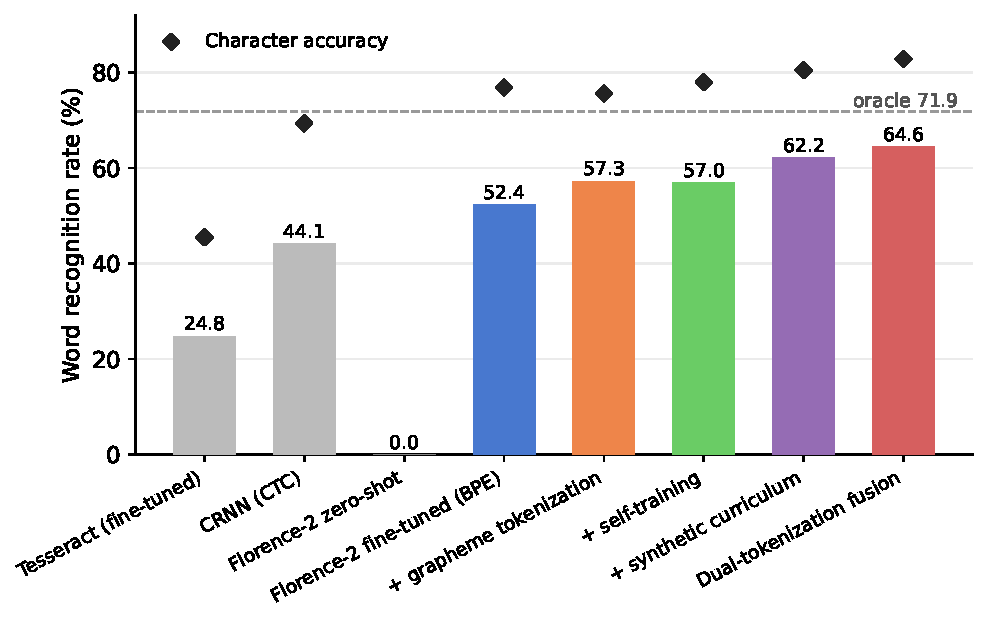
\includegraphics[width=\columnwidth]{fig1_main_results}
\caption{Bengali results. Bars: WRR; diamonds: character accuracy; dashed
line: 4-model oracle ceiling.}
\label{fig:main}
\end{figure}

\subsection{Cross-dataset and cross-script results}
\begin{table}[t]\centering\footnotesize\setlength{\tabcolsep}{3pt}
\caption{BPE vs.\ grapheme vs.\ 2-way fusion across datasets (WRR).
Same recipe, no per-language tuning. Bold = best non-oracle.}
\label{tab:cross}
\begin{tabular}{lccccc}
\toprule
Test set & $n$ & BPE & Grapheme & Fusion & Oracle \\
\midrule
Our Bengali        & 370   & 52.4 & 57.3 & \textbf{59.2} & 64.3 \\
BSTD Bengali       & 1{,}368 & 57.4 & 59.8 & \textbf{62.1} & 66.6 \\
BSTD Assamese      & 1{,}505 & 31.6 & 36.3 & \textbf{38.5} & 43.8 \\
BSTD Hindi         & 4{,}846 & 56.9 & 52.6 & \textbf{61.7} & 66.7 \\
\bottomrule
\end{tabular}
\end{table}

Two regimes emerge (Fig.~\ref{fig:cross}). On the Bengali-script languages,
which the BPE vocabulary covers poorly, the grapheme branch wins
($+4.9$ ours, $+2.4$ BSTD Bengali, $+4.7$ Assamese---the most extreme
low-resource setting, 2{,}365 training words). On Hindi the polarity flips:
Devanagari is far better covered by the BPE vocabulary, and the BPE branch
leads by $4.3$. Critically, fusion beats the \emph{best} branch in both
regimes ($56.9\to61.7$ on Hindi, recovering 49\% of the oracle gap): which
tokenization is stronger varies by script, but their complementarity---and
the reliability of confidence as a selector---does not.

\textbf{Significance.} The grapheme--BPE difference is significant on all
datasets (McNemar $p{=}0.041$ ours, $p{=}0.030$ BSTD Bengali,
$p{=}5{\times}10^{-5}$ Assamese, $p{=}1{\times}10^{-9}$ Hindi). The fusion
gain over the best single branch is significant on the large public test
sets ($p{=}0.0024$ Bengali; $p{=}0.0085$ Assamese; $p{<}10^{-28}$ Hindi,
95\% CI of the gain $[+3.9, +5.6]$) but not powered on our 370-image set
($p{=}0.20$; 95\% CI $[-0.8, +5.7]$)---one reason the public-benchmark
replication is essential, and we report it as such.

\begin{figure}[h]\centering
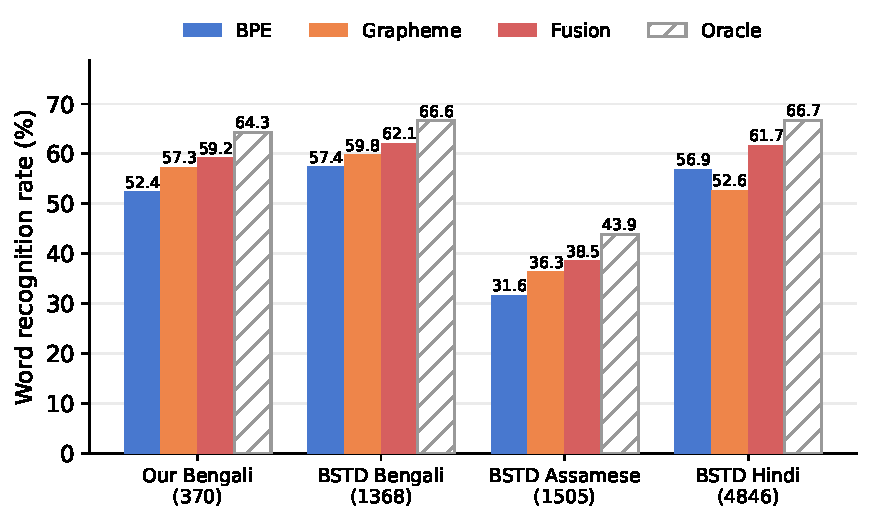
\includegraphics[width=.95\columnwidth]{fig2_cross_dataset}
\caption{Replication of the grapheme advantage and fusion gain across
datasets and scripts.}
\label{fig:cross}
\end{figure}

\subsection{Replication across nine Brahmic scripts}\label{sec:replication}
Do the four test sets above just happen to favor fusion? To test the recipe
at scale we trained BPE and grapheme branches for twelve BSTD languages
under a deliberately uniform protocol---a fixed budget of 1{,}800 real
training words per language, identical hyperparameters, no per-language
tuning---and fused them by max-confidence. Table~\ref{tab:repl} and
Fig.~\ref{fig:repl} report WRR on each language's full real test set.

\begin{table*}[t]\centering\small
\caption{Fixed-budget (1{,}800 train words) replication. $\Delta$ = fusion
minus the better branch; $p$ = exact McNemar, fusion vs.\ better branch.
Fusion wins in 12/12 languages.}
\label{tab:repl}
\begin{tabular}{llccccc}
\toprule
Language & Script & $n$ & BPE & Grph. & Fusion & $\Delta$ \\
\midrule
Punjabi   & Gurmukhi   & 2{,}879  & 54.8 & 44.3 & \textbf{57.8} & $+3.1$ \\
Marathi   & Devanagari & 1{,}196  & 48.7 & 36.8 & \textbf{52.9} & $+4.3$ \\
Odia      & Odia       & 1{,}044  & 33.1 & 47.4 & \textbf{52.4} & $+5.0$ \\
Tamil     & Tamil      & 513      & 28.1 & 36.8 & \textbf{46.4} & $+9.6$ \\
Hindi     & Devanagari & 4{,}846  & 40.8 & 29.8 & \textbf{43.0} & $+2.2$ \\
Telugu    & Telugu     & 545      & 21.3 & 26.8 & \textbf{33.8} & $+7.0$ \\
Gujarati  & Gujarati   & 1{,}015  & 27.1 & 26.7 & \textbf{33.6} & $+6.5$ \\
Bengali   & Bengali    & 1{,}368  & 27.1 & 30.0 & \textbf{31.9} & $+1.8$ \\
Assamese  & Bengali    & 1{,}505  & 26.7 & 27.5 & \textbf{31.6} & $+4.1$ \\
Kannada   & Kannada    & 720      & 21.8 & 23.8 & \textbf{30.8} & $+7.1$ \\
Malayalam & Malayalam  & 547      & 15.2 & 20.8 & \textbf{26.7} & $+5.9$ \\
English   & Latin      & 12{,}568 & 49.0 & 50.8 & \textbf{54.3} & $+3.5$ \\
\bottomrule
\end{tabular}
\end{table*}

\begin{figure*}[t]\centering
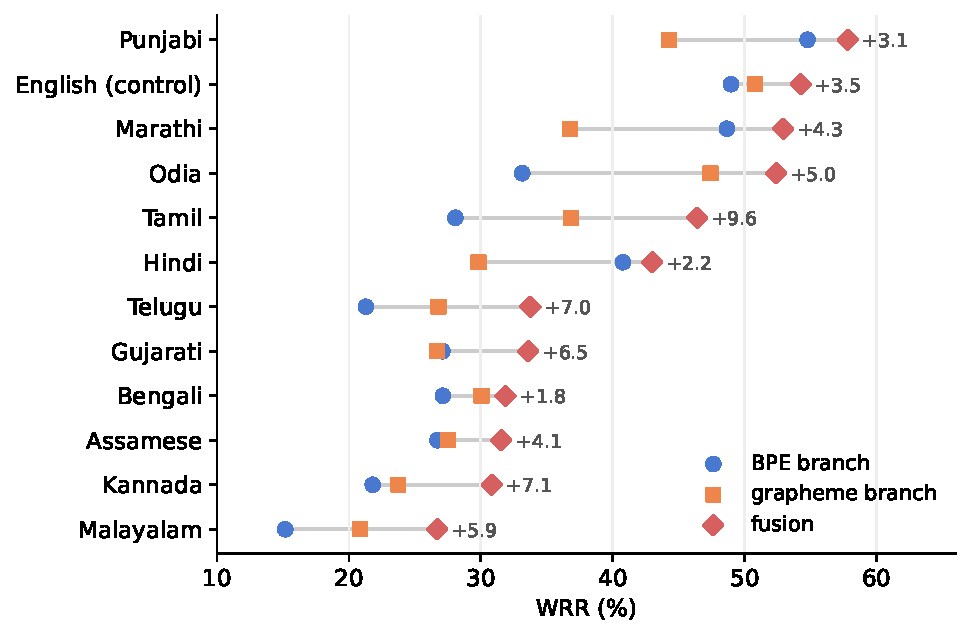
\includegraphics[width=.8\textwidth]{fig8_replication}
\caption{Fixed-budget replication across twelve languages (nine Brahmic
scripts + Latin control), sorted by fusion WRR. The fusion (diamond) is the
rightmost marker in every row; the annotation gives its gain over the
better branch. Note the winning branch flips between rows (BPE ahead on
Punjabi/Marathi/Hindi, grapheme ahead on Odia/Tamil/Telugu/Malayalam,
near-ties on Gujarati/Assamese) while the fusion gain persists.}
\label{fig:repl}
\end{figure*}

Three observations. \emph{First}, fusion exceeds the better single branch
in all twelve languages (mean $+5.0$ WRR), and every gain is individually
significant (exact McNemar; largest $p=0.02$ for Bengali, all others
$p\le 10^{-5}$). \emph{Second}, the winning branch flips with the script:
BPE leads on the scripts best covered by the BPE vocabulary (Devanagari,
Gurmukhi), the grapheme branch leads on Dravidian scripts and Odia, and the
two are statistically indistinguishable on Gujarati and Assamese---where
fusion nonetheless gains $+6.5$ and $+4.1$. A generic two-model ensembling
effect would not exhibit this coverage-tracking structure; the
complementarity is a property of the \emph{tokenizations}. \emph{Third},
the Latin control (English) shows a smaller but real gain ($+3.5$),
indicating the mechanism---confidence arbitrating between differently
tokenized views---is general, while its payoff is largest where the two
tokenizations differ most.

\subsection{Comparison with a large-data specialist recognizer}
\label{sec:parseq}
How does the proposed recipe compare against the strongest available
specialist? We evaluate the BSTD authors' released Bengali PARSeq
model~\cite{bstd,parseq}---pre-trained on \textbf{8.48M synthetic word
images} (SynthText-style rendering) and fine-tuned on the BSTD training
set---on both test sets, under the identical scorer and normalization used
for all systems in this paper (Table~\ref{tab:parseq}).

\begin{table*}[t]\centering\small
\caption{Specialist PARSeq vs.\ our 4-model fusion. PARSeq uses
${\sim}1000\times$ more training data (8.48M synthetic $+$ 4.4k real vs.\
our 7.65k real $+$ 5k synthetic). $p$: exact McNemar on paired correctness.}
\label{tab:parseq}
\begin{tabular}{lcccc}
\toprule
Test set & System & WRR & Char.\ acc. & McNemar $p$ \\
\midrule
\multirow{2}{*}{Our Bengali (370)}
 & PARSeq (transfer) & 66.8 & 84.6 & \multirow{2}{*}{$0.50$} \\
 & Fusion (ours)     & 64.6 & 82.8 & \\
\midrule
\multirow{2}{*}{BSTD Bengali (1{,}368)}
 & PARSeq (in-domain) & 77.3$^{\dagger}$ & 92.9 & \multirow{2}{*}{$<10^{-4}$} \\
 & Fusion (ours)      & 62.1 & 84.1 & \\
\bottomrule
\end{tabular}

\smallskip
{\footnotesize $^{\dagger}$Measured with the authors' released checkpoint
under our protocol; the BSTD paper reports 0.82 under its own protocol. The
0.2-point effect of normalization was verified to be negligible.}
\end{table*}

The comparison is honest in both directions. On its home benchmark the
specialist dominates ($77.3$ vs.\ $62.1$, $p{<}10^{-4}$): large-scale
synthetic pre-training remains the strongest single factor for in-domain
accuracy, and nothing in our method substitutes for it. On our
independently collected test set, however, the transferred specialist is
statistically indistinguishable from our fusion ($66.8$ vs.\ $64.6$,
$p{=}0.50$, 95\% CI of the difference $[-3.2, +7.6]$)---despite the fusion
being trained on three orders of magnitude less data. We therefore position
the contribution as \emph{orthogonal} to data scale: a tokenization-level
finding about VLM recognizers that applies at any data budget, and that
could be combined with large-scale synthetic pre-training---an experiment we
leave to future work.

\subsection{Why fusion works: complementarity and calibration}
\label{sec:calib}
Figure~\ref{fig:comp} decomposes test sets by which branch is correct: on
our Bengali set 11.9\% of images are solved \emph{only} by the grapheme
branch and 7.0\% \emph{only} by BPE---disjoint competence that word-level
selection can harvest. Selection is reliable because confidence is
informative: AUROC of confidence vs.\ correctness is 0.91 (BPE), 0.89
(grapheme), 0.89 (fusion) (Fig.~\ref{fig:calib}). Absolute probabilities
are nonetheless overconfident (ECE 0.32--0.41), so we use confidence only
for \emph{ranking}---which max-confidence fusion, selective prediction,
and the cascade require---never as a probability.

\begin{figure}[h]\centering
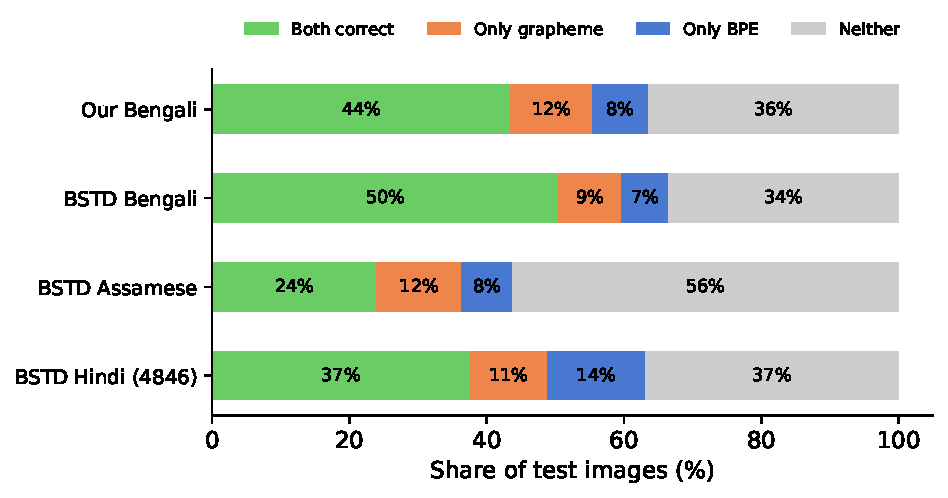
\includegraphics[width=.85\columnwidth]{fig3_complementarity}
\caption{Error complementarity of the BPE and grapheme branches.}
\label{fig:comp}
\end{figure}

\begin{figure*}[t]\centering
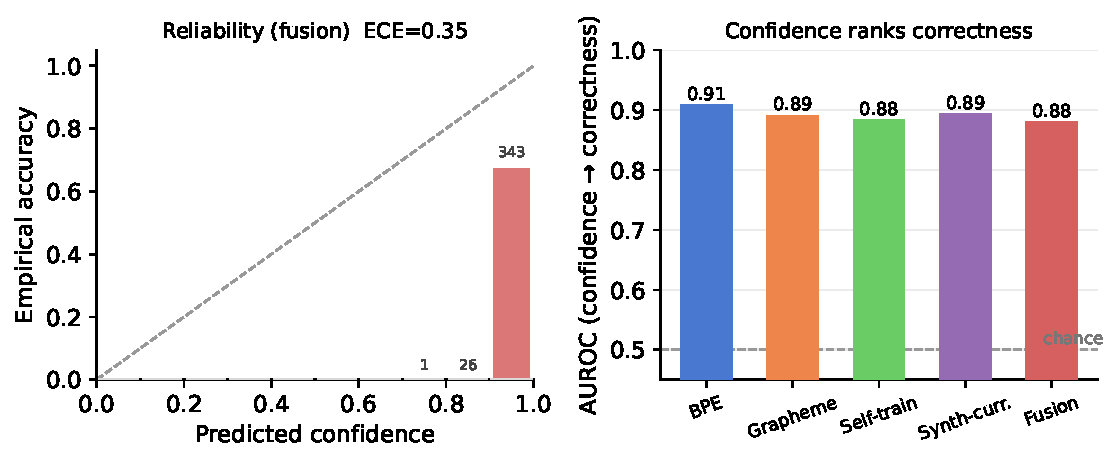
\includegraphics[width=.85\textwidth]{fig5_calibration}
\caption{Left: reliability diagram of the fused system (counts per bin).
Right: confidence ranks correctness (AUROC) for all branches.}
\label{fig:calib}
\end{figure*}

\textbf{Selective prediction.} Ranking by fused confidence and abstaining on
the least-confident images yields 84.9\% WRR at 70\% coverage and 91.4\% at
50\% (Fig.~\ref{fig:risk})---a deployable operating curve for
human-in-the-loop digitization.

\begin{figure}[h]\centering
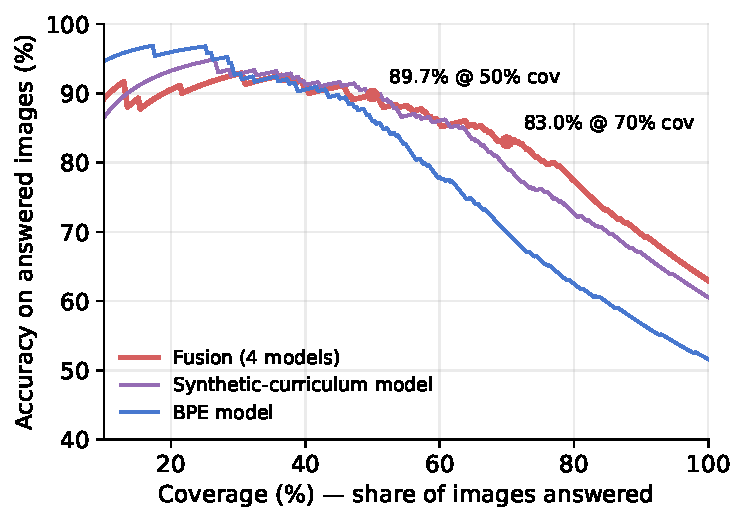
\includegraphics[width=.8\columnwidth]{fig4_risk_coverage}
\caption{Risk--coverage curves on our Bengali test set.}
\label{fig:risk}
\end{figure}

\subsection{Cascaded inference: most of the gain at a fraction of the cost}
\label{sec:cascade}
Table~\ref{tab:cascade} evaluates the cascade of
Sec.~\ref{sec:cascademethod} at a single threshold ($t{=}0.95$) applied
uniformly to all datasets. The grapheme branch is invoked on only
27--58\% of images, yet 66--85\% of the full-fusion WRR gain is retained;
at $t{=}0.99$ the cascade recovers 91--98\% of the gain at a mean decode
cost of ${\sim}1.5\times$. The doubled inference cost of fusion is thus a
tunable deployment knob, not a fixed tax.

\begin{table}[t]\centering\footnotesize\setlength{\tabcolsep}{3pt}
\caption{Cascade at $t{=}0.95$: BPE decodes first; the grapheme branch runs
only when BPE confidence $<t$. ``2nd'' = fraction of images decoded twice;
``gain'' = share of the full-fusion WRR gain retained.}
\label{tab:cascade}
\begin{tabular}{lccccc}
\toprule
Test set & BPE & Fusion & Cascade & 2nd (\%) & gain (\%) \\
\midrule
Our Bengali   & 52.4 & 59.2 & 58.1 & 39 & 84 \\
BSTD Bengali  & 57.4 & 62.1 & 60.5 & 27 & 66 \\
BSTD Assamese & 31.6 & 38.5 & 37.3 & 58 & 82 \\
BSTD Hindi    & 56.9 & 61.7 & 61.0 & 32 & 85 \\
\bottomrule
\end{tabular}
\end{table}

\subsection{Where the gains come from: grapheme rarity}
Bucketing test words by the training frequency of their \emph{rarest}
grapheme (Fig.~\ref{fig:rarity}) shows all models degrade on rare-conjunct
words, but (i) the synthetic curriculum dominates the mid-frequency buckets
it explicitly targets, and (ii) fusion helps most in the rarest bucket
($<$5 occurrences, $n{=}126$: 51.6 vs.\ 40.5 BPE and 46.8 for the best
single model), where single models are least reliable. In the
highest-frequency bucket ($n{=}43$) the curriculum model alone is slightly
ahead of the fusion (88.4 vs.\ 81.4, a 3-word difference, not
significant)---fusion's advantage concentrates exactly where the data is
thin.

\begin{figure}[h]\centering
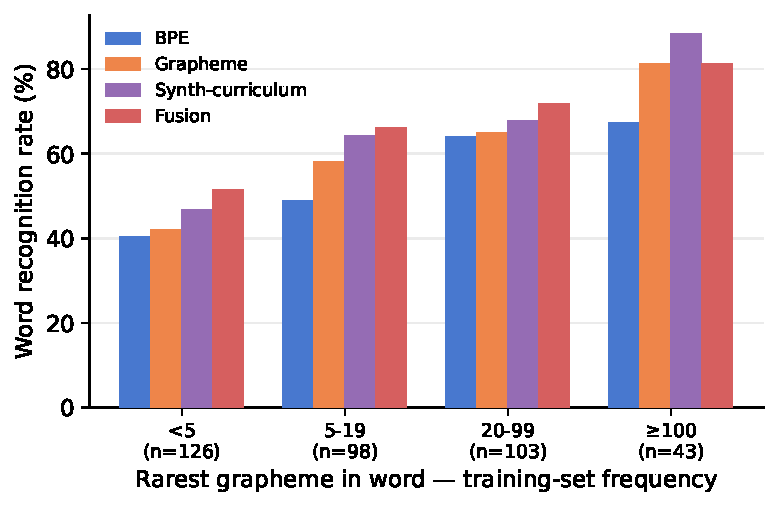
\includegraphics[width=.85\columnwidth]{fig6_rarity_buckets}
\caption{WRR by training-frequency of the rarest grapheme in each test word.}
\label{fig:rarity}
\end{figure}

\subsection{Ablations and negative results}
\textbf{ROVER-style character voting.} Aligning candidates at character
level and voting per slot (confidence-weighted)~\cite{rover} yields 64.05
WRR vs.\ 64.59 for max-confidence on our set, and ties on BSTD; with two
models the vote provably reduces to max-confidence. The simpler rule wins.
\textbf{Self-training} adds character accuracy (+2.3) but not word accuracy
over the grapheme model alone; its value is as a diverse member of the
fusion ensemble. \textbf{Oracle ceilings} (Tables~\ref{tab:main},
\ref{tab:cross}) bound what any selection rule can achieve; remaining errors
are correlated across branches (blur, occlusion, extreme fonts).

\subsection{Qualitative analysis}
Figure~\ref{fig:qual} shows characteristic behavior: the BPE branch
hallucinates plausible-but-wrong subwords on conjunct-heavy words, the
grapheme branch errs on rare whole-word shapes, and fusion selects
correctly; the last panel shows a shared failure under degradation.

\begin{figure*}[t]\centering
\includegraphics[width=.9\textwidth]{fig7_qualitative.png}
\caption{Test crops with ground truth and branch outputs (red = wrong).}
\label{fig:qual}
\end{figure*}

\section{Discussion and limitations}\label{sec:disc}
Absolute WRR remains bounded by data: with $\sim$4k labeled words even the
4-model oracle is 71.9\%, and a specialist trained on 8.48M synthetic words
still dominates in-domain (Sec.~\ref{sec:parseq}); our recipe is a
data-efficiency and tokenization result, not a substitute for scale.
Word-level accuracy above 80\% is achievable today only under selective
prediction; we report this trade-off explicitly rather than as a headline
number. Full fusion doubles inference cost; the cascade of
Sec.~\ref{sec:cascade} reduces this to a tunable trade-off, but the
cheapest deployment remains a single branch. ECE shows confidences are not
calibrated probabilities; all uses in this paper are rank-based. The
twelve-language replication uses a fixed 1{,}800-word budget per language;
budget--accuracy scaling is future work, as are larger backbones
(Florence-2-large) and joint multi-lingual training. Finally, while the
script-dependent polarity flips and the gains on branch-tied languages
(Sec.~\ref{sec:replication}) argue that the fusion harvests
tokenization-specific complementarity rather than generic ensemble
variance reduction, a same-tokenizer multi-seed ensemble control would
isolate this cleanly, and we plan to report it.

\section{Conclusion}\label{sec:conc}
Making a VLM's tokenizer script-aware, then fusing the BPE and grapheme
views by confidence, is a simple, parameter-free recipe that consistently
improves low-resource Indic scene-text recognition---significantly so on
every one of twelve languages spanning nine Brahmic scripts---comes with a
mechanistic explanation (confidence ranks correctness), degrades gracefully
into a reliable selective-prediction system, and needs only a fraction of
its nominal inference cost when cascaded.

\backmatter

\section*{Declarations}
\bmhead{Funding} % FILL: e.g. "This work received no external funding."
FILL BEFORE SUBMISSION.
\bmhead{Competing interests} The authors have no competing interests to
declare that are relevant to the content of this article.
\bmhead{Data availability} The BSTD benchmark is publicly available. Our
Bengali dataset, all train/val/test splits, and per-image predictions with
confidences for every system in this paper will be released upon
publication.
\bmhead{Code availability} Training, evaluation, fusion, and analysis code
(including the script that recomputes every number in this paper from the
released per-image predictions) will be released upon publication.

\begin{thebibliography}{99}\small
\bibitem{crnn} B. Shi, X. Bai, C. Yao. An end-to-end trainable neural
network for image-based sequence recognition and its application to scene
text recognition. IEEE TPAMI 39(11):2298--2304, 2017.
\bibitem{parseq} D. Bautista, R. Atienza. Scene text recognition with
permuted autoregressive sequence models. ECCV 2022.
\bibitem{svtr} Y. Du et al. SVTR: scene text recognition with a single
visual model. IJCAI 2022.
\bibitem{trocr} M. Li et al. TrOCR: transformer-based optical character
recognition with pre-trained models. AAAI 2023.
\bibitem{donut} G. Kim et al. OCR-free document understanding transformer.
ECCV 2022.
\bibitem{florence2} B. Xiao et al. Florence-2: advancing a unified
representation for a variety of vision tasks. CVPR 2024.
\bibitem{indicstr12} H. Lunia, A. Mondal, C.V. Jawahar. IndicSTR12: a
dataset for Indic scene text recognition. ICDAR 2023.
\bibitem{bstd} A. Goswami et al. Bharat Scene Text Dataset (BSTD): a
benchmark for scene text recognition in Indian languages. 2025.
arXiv:2511.23071.
\bibitem{roadside} A. Mondal, K. Tulsyan, C.V. Jawahar. Indic scene text
on the roadside. ICDAR 2024.
\bibitem{lasanet} V.P. Vijayan, S. Chanda, D. Doermann, N.C. Krishnan.
Scene text recognition: an Indic perspective. IJDAR 28:31--40, 2025.
\bibitem{gradet} GraDeT-HTR: grapheme-based decoding transformer for Bengali
handwritten text recognition. EMNLP 2025. arXiv:2509.18081.
\bibitem{mgpstr} P. Wang, C. Da, C. Yao. Multi-granularity prediction for
scene text recognition (MGP-STR). ECCV 2022.
\bibitem{mgpstrj} P. Wang, C. Da, C. Yao. Multi-granularity prediction with
learnable fusion for scene text recognition. IJCV, 2026. arXiv:2307.13244.
\bibitem{lora} E. Hu et al. LoRA: low-rank adaptation of large language
models. ICLR 2022.
\bibitem{selpred} Y. Geifman, R. El-Yaniv. Selective classification for
deep neural networks. NeurIPS 2017.
\bibitem{calib} C. Guo, G. Pleiss, Y. Sun, K.Q. Weinberger. On calibration
of modern neural networks. ICML 2017.
\bibitem{rover} J. Fiscus. A post-processing system to yield reduced word
error rates: recognizer output voting error reduction (ROVER). ASRU 1997.
\end{thebibliography}

\end{document}
